\documentclass[11pt,a4paper]{article}

\usepackage[utf8]{inputenc}
\usepackage[T1]{fontenc}
\usepackage[italian]{babel}
\usepackage[margin=1.8cm]{geometry}
\usepackage{amsmath}
\usepackage{graphicx}
\usepackage{caption}

\captionsetup{font=small,labelfont=bf}
\pagestyle{empty}

\newcommand{\Et}{E_{\mathrm{true}}}
\newcommand{\Er}{E_{\mathrm{rec}}}

\begin{document}

\begin{center}
  {\Large\bfseries Effetto della risoluzione in energia su uno spettro oscillante}
\end{center}

\noindent
Sia $\Et$ l'energia depositata da una particella nel rivelatore e $\Er$ l'energia
ricostruita. Come spettro vero si assume una costante più un'oscillazione di periodo $P$,
nell'intervallo $1~\mathrm{MeV} \le \Et \le 10~\mathrm{MeV}$:
\begin{equation}
  \frac{dN}{d\Et} = 1 + A \sin\!\left(\frac{2\pi \Et}{P}\right),
  \qquad A = 0.8,\quad P = 1~\mathrm{MeV}.
\end{equation}
La risoluzione è descritta da un kernel gaussiano centrato sull'energia vera, la cui
larghezza cresce linearmente con $\Et$, da $5~\mathrm{keV}$ a $1~\mathrm{MeV}$ a
$300~\mathrm{keV}$ a $10~\mathrm{MeV}$:
\begin{equation}
  p(\Er \,|\, \Et) = \frac{1}{\sqrt{2\pi}\,\sigma(\Et)}
  \exp\!\left[-\frac{(\Er-\Et)^2}{2\,\sigma^2(\Et)}\right].
\end{equation}
Lo spettro ricostruito si ottiene con l'integrale di convoluzione a kernel variabile
\begin{equation}
  \frac{dN}{d\Er} = \int_{1\,\mathrm{MeV}}^{10\,\mathrm{MeV}}
  \frac{dN}{d\Et}\; p(\Er \,|\, \Et)\; d\Et ,
\end{equation}
che nella figura è calcolato numericamente. Se $\sigma$ varia lentamente rispetto a $P$,
e lontano dai bordi dell'intervallo, l'integrale si risolve analiticamente:
\begin{equation}
  \frac{dN}{d\Er} \simeq 1 + A\, e^{-2\pi^2\sigma^2(\Er)/P^2}
  \sin\!\left(\frac{2\pi \Er}{P}\right).
\end{equation}
La risoluzione \emph{non modifica il periodo} dell'oscillazione: ne riduce l'ampiezza di
un fattore $e^{-2\pi^2\sigma^2/P^2}$, pari a circa $1$ a $1~\mathrm{MeV}$ e a circa $0.17$
a $10~\mathrm{MeV}$. L'oscillazione si cancella quando $\sigma$ diventa confrontabile con
$P/2\pi$ o maggiore.

\begin{figure}[!htb]
  \centering
  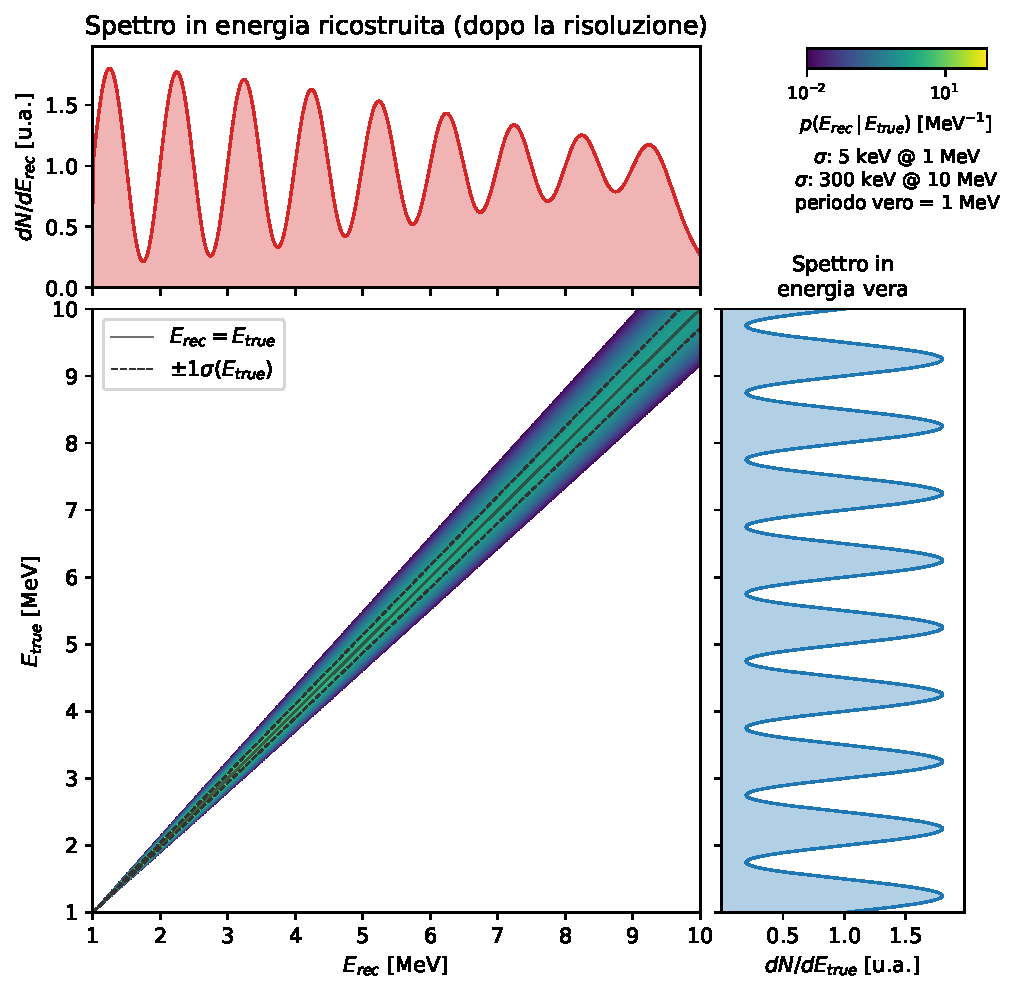
\includegraphics[width=0.52\textwidth]{risoluzione.pdf}
  \caption{\emph{Pannello centrale:} densità di probabilità $p(\Er\,|\,\Et)$ in scala
    logaritmica. Ogni riga orizzontale è la gaussiana associata a un valore di $\Et$. La
    linea continua indica $\Er=\Et$, le linee tratteggiate $\pm1\sigma(\Et)$.
    \emph{Pannello a destra:} spettro vero in funzione di $\Et$.
    \emph{Pannello in alto:} spettro ricostruito in funzione di $\Er$, ottenuto proiettando
    sull'asse $\Er$ il prodotto fra lo spettro vero e il kernel.}
\end{figure}

\noindent
\textbf{Lettura del grafico.} A bassa energia il kernel è molto stretto ($\Er\simeq\Et$) e
lo spettro ricostruito riproduce quello vero. Salendo in energia la banda del kernel si
allarga: ogni valore di $\Er$ riceve contributi da un intervallo di $\Et$ che contiene
massimi e minimi vicini. Picchi e valli si mediano parzialmente, quindi l'ampiezza
dell'oscillazione diminuisce progressivamente mentre la posizione dei massimi, e quindi il
periodo, resta invariata. Vicino a $\Er = 10~\mathrm{MeV}$ lo spettro ricostruito cala
perché gli eventi migrano oltre l'estremo dell'intervallo e mancano eventi con
$\Et > 10~\mathrm{MeV}$ che possano compensarli (effetto di bordo).

\end{document}
